\documentclass[12pt,oneside,a4paper]{article}

\usepackage[utf8]{inputenc} % Lærer LaTeX at forstå unicode - HUSK at filen skal
% være unicode (UTF-8), standard i Linux, ikke i
% Win.

\usepackage[danish]{babel} % Så der fx står Figur og ikke Figure, Resumé og ikke
% Abstract etc. (god at have).

\usepackage{graphicx}
\usepackage{amsfonts}
\usepackage{amsthm}        % Theorems
\usepackage{amsmath}
%\usepackage{hyperref}

%\renewcommand{\mid}[1]{{\rm E}\!\left[#1\right]}
\newcommand{\bas}{\begin{eqnarray*}}
\newcommand{\eas}{\end{eqnarray*}}
\newcommand{\be}{\begin{equation}}
\newcommand{\ee}{\end{equation}}
\newcommand{\bea}{\begin{eqnarray}}
\newcommand{\eea}{\end{eqnarray}}

\theoremstyle{plain}
\newtheorem*{thm}{Sætning}
\newtheorem*{mydef}{Definition}
\newtheorem*{eks}{Eksempel}

\DeclareMathSymbol{,}{\mathord}{letters}{"3B}

\title{Eksponentialfunktioner}
\date{\vspace{-5ex}}

\begin{document}

\maketitle

\section*{Indledning}
Vi kommer til at møde mange forskellige funktioner. Vi har allerede
arbejdet med lineære funktioner. I dette kapitel er emnet eksponentielle
funktioner, og i de næste kapitler vil vi møde bl.a. logaritmefunktioner og
potensfunktioner.

Fælles for alle disse funktioner er, at de har en lang række forskellige
anvendelser. Således optræder eksponentialfunktioner bl.a. inden for økonomi
(rente og rentes rente), biologi (vækst af bakterier og andre organismer),
fysik (radioaktivitet), mm.

\section*{Renteformlen}
\begin{figure}[ht]
    \centering
    
\includegraphics[width=10cm]{penge}
\end{figure}

Vi begynder med et eksempel. Vi har en opsparing på 1000 kroner som vi
indsætter på en opsparingskonto i banken, der giver 5 \% i rente om året. Dvs.
efter 1 år bliver der indsat 5 \% af 1000 kroner på kontoen. Det
udregner vi til $ \frac{5}{100} \cdot 1000 = 50 $ kroner. Så efter 1 år står
der nu 1050 kroner på kontoen.  Efter det andet år bliver der nu indsat 5 \% af
1050 kroner, dvs $ \frac{5}{100} \cdot 1050 = 52,50$ kroner.
Det giver et samlet beløb efter 2 år på 1102,50 kroner. Læg mærke til, at
rentebeløbet det andet år (52,50 kroner) er større end rentebeløbet det første
år (50 kroner).

Hvis vi gerne vil beregne, hvad saldoen bliver efter 8 år, så kan vi fortsætte
ovenstående beregninger. Det er praktisk at opstille beregningerne i et skema
som vist her:
$$
\begin{array}{r|c|l}
    \mbox{efter år} & \mbox{saldo} & \mbox{rentebeløb} \\
    \hline
0 & 1000 & 0,05\cdot 1000 = 50 \\
    \hline
1 & 1050 & 0,05\cdot 1050 = 52,50 \\
    \hline
2 & 1102,50 & 0,05\cdot 1102,50 = 55,13 \\
    \hline
3 & 1157,63 & 0,05\cdot 1157,63 = 57,88 \\
    \hline
4 & 1215,51 & 0,05\cdot 1215,51 = 60,78 \\
    \hline
5 & 1276,29 & 0,05\cdot 1276,29 = 63,81 \\
    \hline
6 & 1340,10 & 0,05\cdot 1340,10 = 67,01 \\
    \hline
7 & 1407,11 & 0,05\cdot 1407,11 = 70,36 \\
    \hline
8 & 1477,47 & 
\end{array}
$$
\begin{figure}[ht]
    \centering
    \includegraphics{eksp-f}
    \label{eksp-f}
\end{figure}
Det vil sige, at efter 8 år, så vil der stå 1477,47 kroner på saldoen.  Dette
er dog en temmelig besværlig metode, og der er en meget nemmere måde at nå frem
til resultatet 1477,47 kroner, hvilket vi skal se i det følgende.

For det første bemærker vi, at for hvert år der går, bliver saldoen ganget med
1,05. Dette kan vi indse ved følgende udregning: Efter det første år bliver
saldoen udregnet som:
$$
1050 = 1000 + 50 = 1000 + 0,05\cdot 1000 = 1,05 \cdot 1000.
$$

Saldoen efter 2 år kan så udregnes som
$$
1,05\cdot 1050 = 1,05 \cdot (1,05 \cdot 1000) = 1,05^2 \cdot 1000.
$$
Saldoen efter 3 år kan på samme måde udregnes som
$$
1,05\cdot1,05\cdot1,05\cdot 1000 = 1,05^3 \cdot 1000.
$$
Efter 8 år er saldoen
derfor på $1,05^8\cdot 1000$. Hvis vi udregner dette på lommeregner, så giver
det netop ca. 1477 kroner.

Denne metode kan udtrykkes ved følgende formel:
\begin{thm}
    {\em Renteformlen} kan udregne saldoen på en opsparing som begynder med
    værdien $K_0$ og som efter hver {\em termin} bliver forøget med en fast
    rente $r$. Saldoen efter $n$ terminer er givet ved følgende formel:
    $$
    K_n = K_0 \cdot (1+r)^n
    $$
    hvor $K_0$ er {\em begyndelseskapitalen}, $r$ er {\em vækstraten}, $n$ er antallet af
    terminer, og $K_n$ er {\em slutkapitalen} efter de $n$ terminer.
\end{thm}
En termin er typisk 1 år, men kan også være f.eks. en måned. Den er bestemt af,
hvor tit der tilskrives et nyt rentebeløb. Vækstraten $r$ er renten udtrykt som
decimaltal. Dvs. hvis renten er 5\%, så er vækstraten $r=\frac{5}{100}=0,05$.

I det følgende gennemgår vi nogle eksempler på anvendelse af renteformlen.
\begin{eks}
    En arv på 20000 kroner indsættes på en opsparingskonto, som
    giver 4\% i rente om året. Hvad vil der stå på kontoen efter 7 år?
\end{eks}
\begin{proof}[Svar]
    Først udregnes vækstraten $r=\frac{4}{100} = 0,04$. Så indsættes i renteformlen:
    $$
    K_7 = 20000 \cdot (1 + 0,04)^7 = 26318,64.
    $$
    Altså efter syv år står der over 26000 kroner på saldoen.
\end{proof}

Renteformlen kan også bruges, når man låner penge, hvis man ikke betaler af
(afdrager) på gælden undervejs.
\begin{eks}
    Hvis en kassekredit har et underskud på 17000 kroner, og der
    lægges 1,8 \% i rente hver måned, hvor meget er gælden så på efter 2 år?
\end{eks}
\begin{proof}[Svar]
    Når renten bliver tilskrevet hver måned, skal de 2 år omregnes til
    måneder, dvs. 24 måneder. Dette er antallet af terminer. Vækstraten er $r =
    \frac{1,8}{100} = 0,018$, og renteformlen giver derfor:
    $$
    K_{24} = 17000 \cdot (1 + 0,018)^{24} = 26085,29
    $$
    Den samlede gæld er derfor vokset til over 26000 kroner på de 2 år, dvs.
    der betales over 7000 i rente.
\end{proof}

\section*{Eksponentialfunktioner}
Renteformlen er et eksempel på en eksponentiel funktion. I det følgende
gennemgår vi en mere generel formel for eksponentialfunktioner, som kan
bruges i mange andre sammenhænge end økonomi.

\subsection*{Forskriften for en eksponentiel funktion}
\begin{mydef}
    En eksponentiel funktion er givet ved følgende forskrift:
    $$
    f(x) = b\cdot a^x
    $$
    hvor $a$ kaldes {\em fremskrivningsfaktoren} og $b$ kaldes {\em
    begyndelsesværdien}. Både $a$ og $b$ skal altid være positive konstanter.
    Definitionsmængden for en eksponentiel funktion er alle tal, dvs. $x$ kan
    være både positiv, negativ og nul; værdimængden er alle positive tal, dvs.
    $f(x)$ er altid positiv.
\end{mydef}

Følgende funktioner er eksempler på eksponentialfunktioner:
$$
\begin{array}{rcll}
    f(x) &=& 3,1 \cdot 1,4^x & ( a=1,4  \, ; \, \, b=3,1) \\
    g(x) &=& 4,7 \cdot 0,91^x & (a=0,91 \, ; \, \, b=4,7) 
\end{array}
$$

\begin{figure}[ht]
    \centering
    \includegraphics{eksp-b}
    \label{eksp-b}
\end{figure}
På figuren ses graferne for disse to funktioner.

\begin{thm}
    Renteformlen svarer til ovenstående definition, hvis man sætter
    \bas
    f(x) = K_n & : & \hbox{værdien efter $n$ terminer.} \\
       b = K_0 & : & \hbox{begyndelsesværdi.} \\
       a = 1+r & : & \hbox{fremskrivningsfaktor.} \\
       x = n   & : & \hbox{antallet af terminer.}
    \eas
\end{thm}

\subsection*{Grafens udseende}
Eksponentialfunktioner er alle monotone; deres monotoniforhold er bestemt af
fremskrivningsfaktoren. Tallene $a$ og $b$ har betydning for, hvordan grafen
ser ud, som det fremgår af følgende:

\begin{itemize}
    \item Hvis $a>1$ er funktionen voksende og grafen krummer opad.
        Når $x$ bliver mindre og mindre, nærmer grafen
        sig $x$-aksen.
    \item Hvis $a<1$ er funktionen aftagende, og grafen nærmer sig
        $x$-aksen, når $x$ bliver større og større.
\end{itemize}

I begge tilfælde siger man også, at $x$-aksen er en vandret {\em asymptote}.
De karakteristiske træk ved eksponentialfunktioner er samlet på figuren.  Læg
mærke til, at grafen aldrig rammer eller krydser $x$-aksen.

\begin{figure}[ht]
    \centering
    \includegraphics{eksp-c}
    \label{eksp-c}
\end{figure}

\begin{thm}
    En eksponentiel funktion vil altid skære $y$-aksen i punktet $(0,\,b)$.
\end{thm}
\begin{proof}
    Dette ses ved at indsætte $x$-koordinaten $x=0$ i forskriften:
    $f(0) = b\cdot a^0 = b\cdot 1 = b$.
\end{proof}

\subsection*{Sproglig formulering}
Eksponentialfunktioner optræder hver gang en størrelse vokser eller falder
med en fast procent.

Det er vigtigt at kunne "oversætte" mellem en sproglig beskrivelse og en matematisk beskrivelse.
I det følgende ser vi på nogle eksempler.

\begin{eks}
    Antallet af ænder i et område er på et tidspunkt målt til 270 ænder. Hvert
    år vokser antallet af ænder med 7 \%. Opskriv en eksponentiel funktion, der
    beskriver udviklingen i antallet af ænder.
\end{eks}
\begin{proof}[Svar]
    Vi kan opskrive følgende formel for antallet af ænder efter $x$ år:
    $$
    f(x) = 270 \cdot 1,07^x
    $$
    Læg mærke til, at fremskrivningsfaktoren er udregnet som $1+\frac{7}{100} =
    1+0,07 = 1,07$.
\end{proof}

\begin{eks}
    Radioaktiviteten af en mængde stof er på et tidspunkt målt til 700. I
    hver time falder strålingen med 3\%. Opskriv en eksponentiel funktion,
    der beskriver udviklingen i radioaktiviteten af stoffet.
\end{eks}
\begin{proof}[Svar]
    Radioaktiviteten efter $x$ timer kan udregnes ved følgende forskrift:
    $$
    f(x) = 700 \cdot 0,97^x
    $$
    Her er fremskrivningsfaktoren udregnet som $1 + \frac{-3}{100} = 1-0,03 = 0,97$.
    Da $a<1$ så betyder det, at radioaktiviteten bliver mindre og mindre med tiden.
\end{proof}

Man skal også kunne oversætte tilbage, dvs fortolke en forskrift. Vi ser på et eksempel:

\begin{eks}
    Antallet af profiler på et nyt socialt medie er givet ved forskriften
    $$
    f(x) = 10000 \cdot 1,27^x
    $$
    hvor $x$ måles i år. Hvad fortæller tallene i forskriften om antallet af
    profiler?
\end{eks}
\begin{proof}[Svar]
    Vi genkender, at der er tale om en eksponentiel funktion med $a=1,27$ og
    $b=10000$.  Disse værdier fortolker vi som, at der til at begynde med er
    10000 profiler på det nye sociale medie, og hvert år bliver der 27 \% flere
    profiler.
\end{proof}

\section*{Regression}
Eksponentialfunktoner bruges også, når man har givet et antal
data-punkter. Et eksempel kunne være nedenstående tabel, som viser det årlige
antal af tvangsopløste selskaber for en række år:
$$
\begin{array}{l|c|c|c|c}
    \mbox{År efter 2006} & 0 & 1 & 2 & 3 \\
    \hline
    \mbox{Antal} & 2180 & 2955 & 3698 & 5530
\end{array}
$$
Tabellen skal læses således, at der f.eks. i år 2009 (3 år efter 2006) blev
opløst i alt 5530 selskaber.

\begin{figure}[ht]
    \centering
    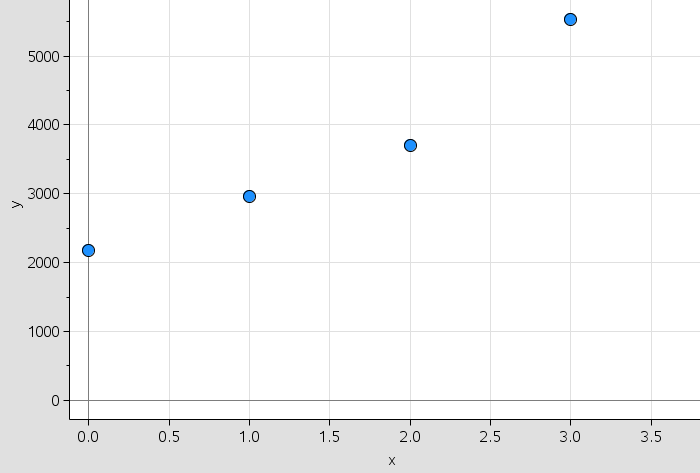
\includegraphics[width=10cm]{eksp-eks1}
\end{figure}

Hvis vi indtegner disse fire punkter i et koordinatsystem, så ser vi en
voksende tendens, som krummer opad. Kan disse data mon beskrives ved en
eksponentiel funktion?

Vi spørger altså, om der findes værdier for tallene $a$ og $b$, som passer med
disse punkter. Det viser sig, at overensstemmelsen ikke er fuldkommen, men at man
med {\em regression} kan finde de værdier af $a$ og $b$, som passer bedst.

På et CAS-værktøj kan man ved hjælp af eksponentiel regression beregne, at
tallene $a$ og $b$ skal have værdierne: 
$$
a = 1,35214\quad,\quad b = 2154,74
$$
Det svarer således til funktionen 
$$
f(x) = 2154,74 \cdot 1,35214 ^x
$$
Tallene i denne forskrift skal fortolkes på følgende måde: I år 2006 var der
ca. 2155 tvangsopløste selskaber, og antallet er siden da vokset med ca. 35 \%
om året.  På næste figur har vi tegnet grafen for denne eksponentialfunktion
og vi kan se, at den passer rimeligt godt med punkterne.

\begin{figure}[ht]
    \centering
    \includegraphics{eksp-e}
    \label{eksp-e}
\end{figure}

Vi siger her, at den eksponentialfunktion er en {\em model} for antallet af
tvangsopløste selskaber. Den gør os i stand til at {\em forudsige}, hvordan
udviklingen vil fortsætte, og beregne værdier mellem tabelpunkterne.

\begin{eks}
    Hvor mange tvangsopløste selskaber vil der være i år 2020?
\end{eks}
\begin{proof}[Svar]
    År 2020 svarer til $x=14$ (14 år efter 2006). Vi udregner:
    $$
    f(14) = 2154,74 \cdot 1,35214^{14} = 147128,9
    $$
    Dette resultat fortolker vi som, at den eksponentielle
    model forudsiger, at ca. 147000 selskaber vil blive tvangsopløst i 2020.
\end{proof}
    

\section*{Vækstegenskaber}
Nu vil vi gå lidt dybere ind i betydningen af fremskrivningsfaktoren. Vi har tidligere
set, at når $x$ stiger med 1, så bliver $f(x)$ ganget med $a$. Dette så vi bl.a. da
vi behandlede rentes rente i begyndelsen af kapitlet.

Som et eksempel på denne type vækst ser vi på den eksponentialfunktion
$$
f(x) = 2,15 \cdot 1,12^x.
$$
Vi laver igen en funktionstabel:
$$
\begin{array}{r|l}
    x & f(x) \\
    \hline
    0 & 2,15 \\
    1 & 2,15 \cdot 1,12^1 = 2,41 \\
    2 & 2,15 \cdot 1,12^2 = 2,70 \\
    3 & 2,15 \cdot 1,12^3 = 3,02
\end{array}
$$
Hvert tal i kolonnen $f(x)$ fremkommer ved at gange det foregående tal med
1,12. F.eks. gælder $2,41 \cdot 1,12 = 2,70$. Det vil sige, at når $x$ stiger
med 1, så bliver $f(x)$ ganget med 1,12.

Hved sker der mon så, hvis $x$ stiger med 2? Svar: Så bliver $f(x)$ ganget med
$1,12^2 = 1,25$.  Det kan vi kontrollere i ovenstående tabel ved at udregne
$2,15\cdot1,25 = 2,69$ og $2,41\cdot1,25 = 3,01$, som passer bortset fra afrunding på
sidste decimal.

Der gælder helt generelt, at hver gang $x$ stiger med en fast værdi, så bliver
$f(x)$ ganget med en fast faktor. Dette er beskrevet i følgende sætning:

\begin{thm}
    For en eksponentiel funktion $f(x) = b\cdot a^x$ gælder: Hvis $x$ ændres
    med en fast værdi $h$, så ganges $f(x)$ med en fast faktor $a^h$.
\end{thm}
\begin{proof}
    For en hvilken som helst konstant $h$ har vi
    $$
    f(x+h) = b\cdot a^{x+h} = b\cdot a^x\cdot  a^h = f(x)\cdot  a^h
    $$
    hvilket viser, at når $x$ ændres med $h$, så bliver $f(x)$ ganget med
    faktoren $a^h$. 
\end{proof}

\begin{eks}
    Vi ser på $f(x) = 21,5 \cdot 1,2^x$ og ønsker at svare på følgende
    spørgsmål: Hvor meget vokser $f(x)$ med, når $x$ vokser med $3,1$?
\end{eks}
\begin{proof}[Svar]
    Vi benytter sætningen ovenfor med $h=3,1$ og udregner derfor:
    $$
    1,2^{3,1} = 1,76 
    $$
    Funktionsværdien $f(x)$ bliver altså ganget med faktoren 1,76, hvilket
    svarer til, at $f(x)$ vokser med $76\%$.
\end{proof}


\section*{Eksponentiel funktion fastlagt ved to punkter}
Hvis man kun kender to punkter, der ikke har samme $x$-værdi, så vil der være
netop én eksponentiel funktion,
hvis graf går gennem de to punkter. Dette er samme situation som ved lineære
funktioner.

Vi viser først ved et eksempel, hvordan man kan bestemme værdierne for tallene
$a$ og $b$, når man kender koordinaterne for de to punkter.
Hvis vi vil bestemme den eksponentialfunktion $f(x) = b\cdot a^x$, der har en
graf, der går igennem punkterne $(3, 2)$ og $(5, 18)$, kan vi gå frem på
følgende måde:
Da grafen for $f(x)$ går igennem de to punkter, er $f(3) = 2$ og $f(5) = 18$. Dvs.
\bas
b \cdot a^3  &=& 2\\
b \cdot a^5  &=& 18
\eas
Ved at isolere $b$ i den første ligning får vi
$$
b = \frac{2}{a^3}
$$
Dette indsættes i den anden ligning:
$$
\frac{2}{a^3} \cdot a^5 = 18
$$
som omskrives til
$$
\frac{2 \cdot a^5}{a^3} = 18
$$
Nu divideres med 2 på begge sider:
$$
\frac{a^5}{a^3} = 9
$$
og vi benytter en potensregneregel til at reducere:
$$
a^2 = 9
$$
og vi ser, at $a=3$ er den eneste løsning, fordi $a$ skal være positiv.

Derefter finder vi, at 
$$
b = \frac{2}{3^3} = \frac{2}{27}
$$

Vi har således fundet frem til, at der er netop én eksponentiel funktion gennem
de to givne punkter, og den har forskriften (se også figuren):
$$
f(x) = \frac{2}{27} \cdot 3^x
$$

\begin{figure}[ht]
    \centering
    \includegraphics{eksp-d}
    \label{eksp-d}
\end{figure}

Denne metode er beskrevet i følgende sætning:

\begin{thm}
    Hvis grafen for en eksponentiel funktion går gennem de to punkter $(x_1,
    \,y_1)$ og $(x_2, \,y_2)$, så er tallene $a$ og $b$ givet ved:
    $$
    a = \left(\frac{y_2}{y_1}\right)^{\frac{1}{x_2-x_1}}
    $$
    og
    $$
    b = \frac{y_1}{a^{x_1}}
    $$
\end{thm}
\begin{proof}
    At funktionen går gennem punktet $(x_1, \,y_1)$ betyder, at $y_1 = f(x_1)$
    og tilsvarende for punktet $(x_2,\,y_2)$. Ved at indsætte den generelle
    forskrift for en eksponentiel funktion, så giver det:
    $$
    y_1 = b\cdot a^{x_1}
    $$
    og 
    $$
    y_2 = b \cdot a^{x_2}
    $$
    Dette er to ligninger med de to ubekendte $a$ og $b$. For at løse disse ligninger
    isolerer vi $b$ i den første ligning. Det giver:
    $$
    b = \frac{y_1}{a^{x_1}}
    $$
    Dette indsættes i den anden ligning, og så omskrives resultatet:
    \bas
    y_2 &=& \frac{y_1}{a^{x_1}} \cdot a^{x_2} \\
    &=& \frac{y_1 \cdot a^{x_2}}{a^{x_1}} \\
    &=& y_1 \cdot \frac{a^{x_2}}{a^{x_1}} \\
    &=& y_1 \cdot a^{x_2-x_1}
    \eas
    Nu kan vi dividere med $y_1$:
    $$
    \frac{y_2}{y_1} = a^{x_2-x_1},
    $$
    og til sidst opløftes begge sider i potensen $\frac{1}{x_2-x_1}$:
    $$
    \left(\frac{y_2}{y_1}\right)^{\frac{1}{x_2-x_1}} = a
    $$
\end{proof}

\end{document}

